% GENERATED BY sshrc_figures.py - edit that file, not this one.
% The document that inputs this file supplies the float, the caption and the label.
% Stream A. Committees, left to right within each year: Philosophy, History, Fine arts, Literature, Sociology, Geography, Psychology (10A, 10B), Political science, Education (12A, 12B, 12C), Anthropology, Linguistics, Communications, Law and criminology.
\definecolor{sshrcA}{HTML}{2A78D6}
\definecolor{sshrcB}{HTML}{EB6834}
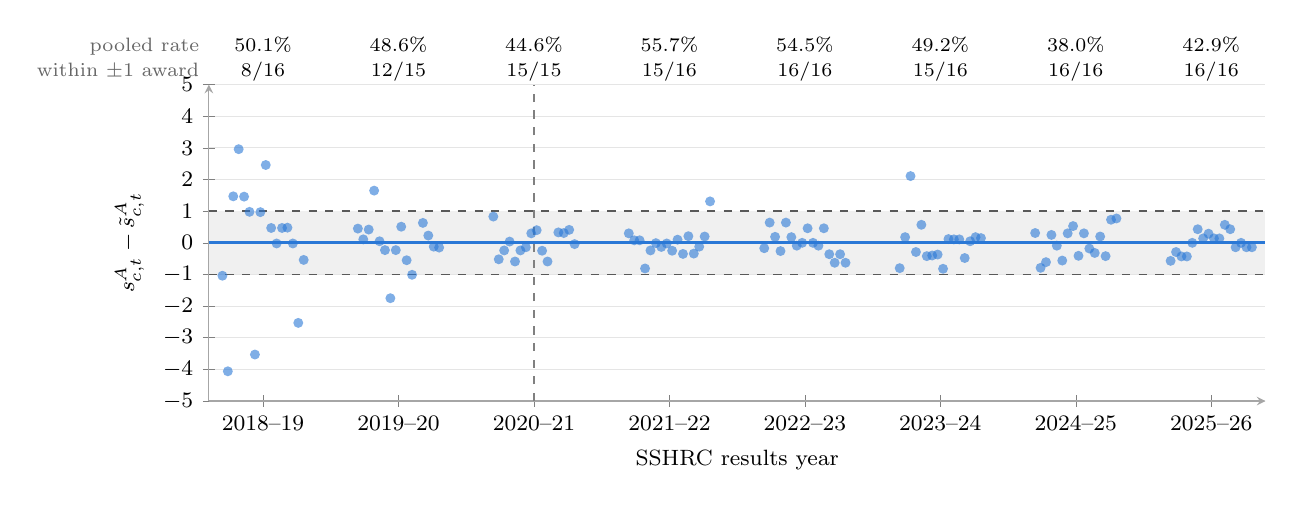
\begin{tikzpicture}
\begin{axis}[
  width=15cm, height=5.6cm,
  xmin=2017.6, xmax=2025.4, ymin=-5, ymax=5,
  xtick={2018,2019,2020,2021,2022,2023,2024,2025}, xticklabels={2018--19,2019--20,2020--21,2021--22,2022--23,2023--24,2024--25,2025--26},
  axis x line=bottom, axis y line=left, axis line style={gray!70},
  ymajorgrids, grid style={gray!20},
  tick label style={font=\footnotesize}, label style={font=\footnotesize},
  xlabel={SSHRC results year}, ylabel={$s^{A}_{c,t}-\tilde{s}^{A}_{c,t}$}, ylabel style={align=center},
  clip=false,
  ytick distance=1,
]
\fill[gray!12] (axis cs:2017.6,-1) rectangle (axis cs:2025.4,1);
\draw[gray, dashed, line width=0.7pt] (axis cs:2020,-5) -- (axis cs:2020,5);
\addplot[color=sshrcA, line width=1.2pt, forget plot, domain=2017.6:2025.4, samples=2] {0};
\addplot[gray!70!black, line width=0.7pt, dashed, forget plot, domain=2017.6:2025.4, samples=2] {-1};
\addplot[gray!70!black, line width=0.7pt, dashed, forget plot, domain=2017.6:2025.4, samples=2] {1};
\addplot[only marks, mark=*, mark size=1.8pt, color=sshrcA,
  mark options={fill opacity=0.6, draw opacity=0}]
  coordinates {(2018.18,0.48) (2018.26,-2.53) (2018.06,0.47) (2018.10,-0.02) (2018.14,0.47) (2017.78,1.47) (2017.90,0.98) (2017.74,-4.06) (2018.30,-0.54) (2018.22,-0.02) (2017.82,2.96) (2017.70,-1.04) (2018.02,2.46) (2017.94,-3.53) (2017.98,0.97) (2017.86,1.46) (2019.18,0.63) (2019.26,-0.12) (2019.06,-0.55) (2019.10,-1.01) (2018.78,0.42) (2018.90,-0.23) (2018.74,0.11) (2019.30,-0.15) (2019.22,0.23) (2018.82,1.65) (2018.70,0.45) (2019.02,0.51) (2018.94,-1.75) (2018.98,-0.23) (2018.86,0.05) (2019.70,0.83) (2019.74,-0.52) (2019.78,-0.24) (2019.82,0.04) (2019.86,-0.59) (2019.90,-0.24) (2019.94,-0.14) (2019.98,0.30) (2020.02,0.40) (2020.06,-0.25) (2020.10,-0.59) (2020.18,0.33) (2020.22,0.31) (2020.26,0.41) (2020.30,-0.04) (2020.70,0.30) (2020.74,0.08) (2020.78,0.08) (2020.82,-0.81) (2020.86,-0.24) (2020.90,-0.01) (2020.94,-0.13) (2020.98,-0.02) (2021.02,-0.25) (2021.06,0.10) (2021.10,-0.35) (2021.14,0.21) (2021.18,-0.34) (2021.22,-0.12) (2021.26,0.20) (2021.30,1.31) (2021.70,-0.17) (2021.74,0.64) (2021.78,0.19) (2021.82,-0.26) (2021.86,0.64) (2021.90,0.18) (2021.94,-0.09) (2021.98,0.00) (2022.02,0.46) (2022.06,0.00) (2022.10,-0.09) (2022.14,0.46) (2022.18,-0.36) (2022.22,-0.63) (2022.26,-0.36) (2022.30,-0.63) (2022.70,-0.80) (2022.74,0.18) (2022.78,2.11) (2022.82,-0.29) (2022.86,0.57) (2022.90,-0.42) (2022.94,-0.40) (2022.98,-0.37) (2023.02,-0.82) (2023.06,0.12) (2023.10,0.11) (2023.14,0.11) (2023.18,-0.48) (2023.22,0.05) (2023.26,0.18) (2023.30,0.15) (2023.70,0.31) (2023.74,-0.79) (2023.78,-0.61) (2023.82,0.25) (2023.86,-0.09) (2023.90,-0.56) (2023.94,0.30) (2023.98,0.53) (2024.02,-0.41) (2024.06,0.30) (2024.10,-0.18) (2024.14,-0.32) (2024.18,0.20) (2024.22,-0.42) (2024.26,0.73) (2024.30,0.77) (2024.70,-0.57) (2024.74,-0.29) (2024.78,-0.43) (2024.82,-0.43) (2024.86,0.00) (2024.90,0.43) (2024.94,0.14) (2024.98,0.29) (2025.02,0.14) (2025.06,0.14) (2025.10,0.57) (2025.14,0.43) (2025.18,-0.14) (2025.22,0.00) (2025.26,-0.14) (2025.30,-0.14)};
\node[font=\scriptsize, anchor=base east, text=gray!80!black] at ([yshift=12pt]axis cs:2017.6,5) {pooled rate};
\node[font=\scriptsize, anchor=base] at ([yshift=12pt]axis cs:2018,5) {50.1\%};
\node[font=\scriptsize, anchor=base] at ([yshift=12pt]axis cs:2019,5) {48.6\%};
\node[font=\scriptsize, anchor=base] at ([yshift=12pt]axis cs:2020,5) {44.6\%};
\node[font=\scriptsize, anchor=base] at ([yshift=12pt]axis cs:2021,5) {55.7\%};
\node[font=\scriptsize, anchor=base] at ([yshift=12pt]axis cs:2022,5) {54.5\%};
\node[font=\scriptsize, anchor=base] at ([yshift=12pt]axis cs:2023,5) {49.2\%};
\node[font=\scriptsize, anchor=base] at ([yshift=12pt]axis cs:2024,5) {38.0\%};
\node[font=\scriptsize, anchor=base] at ([yshift=12pt]axis cs:2025,5) {42.9\%};
\node[font=\scriptsize, anchor=base east, text=gray!80!black] at ([yshift=3pt]axis cs:2017.6,5) {within $\pm1$ award};
\node[font=\scriptsize, anchor=base] at ([yshift=3pt]axis cs:2018,5) {8/16};
\node[font=\scriptsize, anchor=base] at ([yshift=3pt]axis cs:2019,5) {12/15};
\node[font=\scriptsize, anchor=base] at ([yshift=3pt]axis cs:2020,5) {15/15};
\node[font=\scriptsize, anchor=base] at ([yshift=3pt]axis cs:2021,5) {15/16};
\node[font=\scriptsize, anchor=base] at ([yshift=3pt]axis cs:2022,5) {16/16};
\node[font=\scriptsize, anchor=base] at ([yshift=3pt]axis cs:2023,5) {15/16};
\node[font=\scriptsize, anchor=base] at ([yshift=3pt]axis cs:2024,5) {16/16};
\node[font=\scriptsize, anchor=base] at ([yshift=3pt]axis cs:2025,5) {16/16};
\end{axis}
\end{tikzpicture}
